\documentclass[mathserif]{beamer}

\usepackage{parskip}
\usepackage{amsmath}
\usepackage{amssymb}
\usepackage{graphicx}

\frenchspacing

\logo{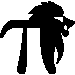
\includegraphics[width=0.075\textwidth]{../Logo}}

\usetheme{Rochester}
\usecolortheme{whale}
%\beamertemplatenavigationsymbolsempty

\AtBeginSection[] {%
	\begin{frame}
		\frametitle{Table of Contents}
		\tableofcontents[currentsection]
	\end{frame}
}

\newenvironment{compactmath}[1][\normalsize]%
	{\begin{minipage}{\textwidth}\vspace{-0.75\baselineskip}#1\begin{equation*}}
	{\end{equation*}\end{minipage}}

\newenvironment{namedframe}[1]%
	{\begin{frame}\frametitle{#1}\framesubtitle{\secname}}
	{\end{frame}}


\usepackage{siunitx}

\title{Geometry 1}
\author{Caroline Liu}
\date{
\includegraphics{../LicenseLogo}\\\copyright{} Caroline Liu, 2017}

\begin{document}
	\frame{\titlepage}
	\section{Introduction}
	\begin{namedframe}{Polygons}
		Polygons are 2D shapes that have 3 or more sides.
		\pause

		Polygons are named after the number of sides the shape has.
		\pause

		\begin{center}
			\begin{tabular}{|c|c|c|}
				\hline
				Sides & Prefix & Name\\\hline
				3     & Tri    & Triangle\\
				4     & Quad   & Quadrilateral\\
				5     & Penta  & Pentagon\\\hline
			\end{tabular}
		\end{center}
	\end{namedframe}
	\begin{namedframe}{Angles}
		The sum of a shape's interior angles can be found with this formula:
		\[\frac{180(n-2)}{n}\]
		\pause

		The sum of a shape's exterior angles can be found with this formula:
		\[360\si{\degree}\]
		(It's always \SI{360}{\degree}.)
		\pause

		These formulas are \alert{very} useful for contests.
	\end{namedframe}
	\begin{namedframe}{Shapes to look out for: without 3 sides}
		\begin{description}[<+->]
			\item[Trapezoids] Can often be split into 2 triangles and a rectangle. Questions include determining a dimension given other info, or calculating area. Very common contest question.
			\item[Parallelograms, squares, and rectangles] May be used in conjunction with circles, or you will be tasked with finding a dimension given some info. Also a common contest question.
		\end{description}
	\end{namedframe}
	\section{Triangles}
	\begin{namedframe}{Facts, formulas, and things to look out for}
		Triangles are one of the most common shapes found on contests. Whether it’s determining angles or sides, or deducing similar triangles, they are almost a guarantee. Basic concepts needed are the sum of the interior angles being \SI{180}{\degree}, and that the sum of 2 sides should never be larger than the 3rd side
		\pause

		Next, we'll go over some important concepts.
	\end{namedframe}
	\section{Pythagorean theorem}
	\begin{namedframe}{Your best friend}
	\end{namedframe}
	\section{Important/special triangles}
	\begin{namedframe}{Pythagorean triplets}
	\end{namedframe}
	\begin{namedframe}{Other nice numbers}
	\end{namedframe}
	\section{Trigonometric identities}
	\begin{namedframe}{SOHCAHTOA}
	\end{namedframe}
	\begin{namedframe}{Cheat sheet}
	\end{namedframe}
	\section{Similar triangles}
	\begin{namedframe}{What similar triangles are}
	\end{namedframe}
	\begin{namedframe}{Conditions for similarity}
	\end{namedframe}
	\section{Special lines and points of intersection}
	\begin{namedframe}{Special lines}
	\end{namedframe}
	\begin{namedframe}{Special points of intersection}
	\end{namedframe}
	\begin{namedframe}{Special POI properties}
	\end{namedframe}
\end{document}
